% -*- root: Proposal.tex -*-
\documentclass[Proposal.tex]{subfiles} 
\begin{document}
\chapter{Implicit Time Stepping with DPG}
The proposed research into space-time DPG does not imply that DPG is incompatible with other time integration techniques. 
We did spend some time exploring popular alternatives such as some ESDIRK (explicit first step singly diagonal implicit Runge-Kutta) methods 
before we ultimately concluded that a space-time formulation might more naturally fit with our adaptive techniques.
In this chapter, we briefly outline some of our exploratory work on implicit time integrators with DPG.


We wish to solve the system
\[
\frac{\partial U}{\partial t}+f(U)=0\,.
\]
It is not immediately clear how one could perform explicit time-stepping with DPG since an explicit system has 
$f(U)$ on the right hand side, but the DPG traces and fluxes are included in the $f(U)$ term and thus need to be solved for.
So moving forward, we focus on implicit techniques which also have superior stability properties.

\section{Backward Euler}
The simplest implicit time stepping method would be backward Euler, for which we get the following system to solve at each time step $n$:
\begin{equation}
	\frac{U^{n}}{\Delta t}+f(U^{n})=\frac{U^{n-1}}{\Delta t}\,,
\end{equation}
where $U^{n-1}$ is known data from the previous time step, and $\Delta t$ is the time step. 
In general, $f(U^n)$ could be nonlinear, in which case we define a residual
\begin{equation}
	R(U^n)=\frac{U^n}{\Delta t}+f(U^n)-\frac{U^{n-1}}{\Delta t}\,.
\end{equation}
Given an approximate solution $\tilde U^n$, we wish to solve for an increment $\Delta U$ such that $U^n=\tilde U^n+\Delta U$ is a better approximation of the true solution.
Approximating $R(U^n)=0$ by $R(\tilde U^n)+R'(\tilde U^n)\Delta U=0$, where $R'(\tilde U^n)$ is the Jacobian of $R$ at $\tilde U^n$, we obtain a linear equation
\begin{equation}
\frac{\Delta U}{\Delta t}+f'(\tilde U)\Delta U
=\frac{U_n}{\Delta t}-\frac{\tilde U}{\Delta t}
-f(\tilde U)\,.
\end{equation}
Note that $f(\tilde U)$ only contains terms that had to be linearized. In general, we do not need to linearize our flux and trace terms in DPG, and hence those terms are excluded from $f(\tilde U)$.

%   /$$$$$$$$  /$$$$$$  /$$$$$$$  /$$$$$$ /$$$$$$$  /$$   /$$
%  | $$_____/ /$$__  $$| $$__  $$|_  $$_/| $$__  $$| $$  /$$/
%  | $$      | $$  \__/| $$  \ $$  | $$  | $$  \ $$| $$ /$$/ 
%  | $$$$$   |  $$$$$$ | $$  | $$  | $$  | $$$$$$$/| $$$$$/  
%  | $$__/    \____  $$| $$  | $$  | $$  | $$__  $$| $$  $$  
%  | $$       /$$  \ $$| $$  | $$  | $$  | $$  \ $$| $$\  $$ 
%  | $$$$$$$$|  $$$$$$/| $$$$$$$/ /$$$$$$| $$  | $$| $$ \  $$
%  |________/ \______/ |_______/ |______/|__/  |__/|__/  \__/
%                                                            
%                                                            
%                        
\section{ESDIRK}
After a literature search, ESDIRK time stepping schemes were identified as a potentially attractive high order time integration technique to couple with DPG.
From an implementation point of view, ESDIRK schemes are much simpler to implement than full implicit Runge-Kutta schemes since each stage may be computed in sequence rather than as a fully coupled system. 
This cuts down on the number of unknowns to keep track of, reducing memory requirements.
The ``explicit first stage'' is completely trivial, requiring no work at all. 
This reduces a formally $s$-stage scheme to $s-1$ stages of actual computational work.
Finally, the final stage coincides with the desired value at the $n$th time step, eliminating the need to have a final reconstruction step.
A 6 stage ESDIRK algorithm has the following Butcher tableau:
\[
\begin{array}{c|cccccc}
  0 & 0 & 0 & 0 & 0 & 0 & 0 \\
  c_1 & a_{10} & a_{11} & 0 & 0 & 0 & 0 \\
  c_2 & a_{20} & a_{21} & a_{22} & 0 & 0 & 0 \\
  c_3 & a_{30} & a_{31} & a_{32} & a_{33} & 0 & 0 \\
  c_4 & a_{40} & a_{41} & a_{42} & a_{43} & a_{44} & 0 \\
  c_5 & a_{50} & a_{51} & a_{52} & a_{53} & a_{54} & a_{55} \\
  \hline
   & b_0 & b_1 & b_2 & b_3 & b_4 & b_5 \\
\end{array}
\begin{array}{c}
  \vphantom{} \\
  \vphantom{} \\
  \vphantom{} \\
  \vphantom{} \\
  \vphantom{} \\
  \vphantom{} \\
  . \\
\end{array}
\]

From a stability point of view, ESDIRK schemes provide both A-stability and L-stability. 
The more classical backwards differentiation formula are not A-stable above second order.
ESDIRK schemes enforce a ``stiffly accurate'' assumption that $a_{sj}=b_j$ which makes the solution at the next time step $U^n$ independent of any explicit process within the integration step.
There is also precedence for using ESDIRK schemes with fluid dynamics simulations (see \cite{Bijl2002}, where ESDIRK schemes were found to be more efficient than BDF schemes for laminar flow over a cylinder).

\subsection{ESDIRK with DPG}
For an $s$ stage ESDIRK scheme, we solve a series of equations for $k=0,\cdots,s-1$
\begin{equation*}
\frac{U^k}{a_{kk}\Delta t}+f(U^k)=\frac{U_n}{a_{kk}\Delta
t}-\sum_{j=0}^{k-1}\frac{a_{kj}}{a_{kk}}f(U^j)\,.
\end{equation*}
From the first equation we see that $U^0=U_n$. And we have that $U_{n+1}=U^s$.
For a nonlinear system, define residual
\[
R(U^k) =
\frac{U^k}{a_{kk}\Delta t}+f(U^k)-\frac{U_n}{a_{kk}\Delta
t}+\sum_{j=0}^{k-1}\frac{a_{kj}}{a_{kk}}f(U^j)
\]
Utilizing the same linearization as above, we arrive at our linearized system
\begin{equation}
	\label{eq:ESDIRKScheme}
	\frac{\Delta U}{a_{kk}\Delta t}+f'(\tilde U^k)\Delta U
	=\frac{U_n}{a_{kk}\Delta t}-\frac{\tilde U^k}{a_{kk}\Delta t}-f(\tilde U^k)
	-\sum_{j=0}^{k-1}\frac{a_{kj}}{a_{kk}}f(U^j)\,,
	\end{equation}
which is to be solved iteratively at each stage until $R(\tilde U^k)$ is smaller than some tolerance.
Note that contrary to the $f(\tilde U)$ term which comes from the linearization and excludes flux and trace terms,
$f(U^j)$ will need to keep the flux and trace terms from the DPG bilinear form.
It is worth noting that terms necessary to construct $f(U^0)$ might not available from the initial condition because they include traces and fluxes.
It is certainly possible to initialize the fluxes and traces for the initial condition, but it is not quite as convenient as setting the field variables.
Thus in the following numerical experiment, we kick start the simulation with a backward Euler solve on a time step one thousandth the size of requested time step before switching fully to the ESDIRK scheme.

%   /$$$$$$$                                                             
%  | $$__  $$                                                            
%  | $$  \ $$ /$$   /$$  /$$$$$$   /$$$$$$   /$$$$$$   /$$$$$$   /$$$$$$$
%  | $$$$$$$ | $$  | $$ /$$__  $$ /$$__  $$ /$$__  $$ /$$__  $$ /$$_____/
%  | $$__  $$| $$  | $$| $$  \__/| $$  \ $$| $$$$$$$$| $$  \__/|  $$$$$$ 
%  | $$  \ $$| $$  | $$| $$      | $$  | $$| $$_____/| $$       \____  $$
%  | $$$$$$$/|  $$$$$$/| $$      |  $$$$$$$|  $$$$$$$| $$       /$$$$$$$/
%  |_______/  \______/ |__/       \____  $$ \_______/|__/      |_______/ 
%                                 /$$  \ $$                              
%                                |  $$$$$$/                              
%                                 \______/       
\subsection{Case Study: 2D Burgers' Equation}
We consider the 2D Burger's equations and accompanying problem outlined in \cite{Burgers2D}.
The 2D Burgers' equations are:
\begin{equation}
	\begin{aligned}
		\frac{\partial u_1}{\partial t}+u_1\frac{\partial u_1}{\partial x}+u_2\frac{\partial u_1}{\partial y}-\frac{1}{R}\Delta u_1&=0\\
		\frac{\partial u_2}{\partial t}+u_1\frac{\partial u_2}{\partial x}+u_2\frac{\partial u_2}{\partial y}-\frac{1}{R}\Delta u_2&=0\,,
	\end{aligned}
\end{equation}
where $R$ is the effective Reynolds number.

\subsubsection{DPG Formulation}
As a first order system, this is
\begin{equation}
	\begin{aligned}
		R\bfsigma_1-\Grad u_1&=0\\
		R\bfsigma_2-\Grad u_2&=0\\
		\frac{\partial u_1}{\partial t}+R\vecttwo{u_1}{u_2}\cdot\bfsigma_1-\Div\bfsigma_1&=0\\
		\frac{\partial u_2}{\partial t}+R\vecttwo{u_1}{u_2}\cdot\bfsigma_2-\Div\bfsigma_2&=0\,.
	\end{aligned}
\end{equation}
Multiplying by test functions $\bftau_1$, $\bftau_2$, $v_1$, $v_2$, and integrating by parts:
\begin{equation}
\label{eq:Burgers2DBF}
	\begin{aligned}
		\LRp{R\bfsigma_1,\bftau_1}+\LRp{u_1,\Div\bftau_1}-\LRa{\hat u_1,\tau_{1n}}&=0\\
		\LRp{R\bfsigma_2,\bftau_2}+\LRp{u_2,\Div\bftau_2}-\LRa{\hat u_2,\tau_{2n}}&=0\\
		\LRp{\frac{\partial u_1}{\partial t},v_1}+\LRp{R\vecttwo{u_1}{u_2}\cdot\bfsigma_1,v_1}+\LRp{\bfsigma_1,\Grad v_1}-\LRa{\hat t_1,v_1}&=0\\
		\LRp{\frac{\partial u_2}{\partial t},v_2}+\LRp{R\vecttwo{u_1}{u_2}\cdot\bfsigma_2,v_2}+\LRp{\bfsigma_2,\Grad v_2}-\LRa{\hat t_2,v_2}&=0\,,
	\end{aligned}
\end{equation}
where it is clear that $v_1,v_2\in\HOneK$, and $\bftau_1,\bftau_2\in\HdivK$. 
In order to plug this into \eqref{eq:ESDIRKScheme}, we need to identify $f(U^j)$, $f(\tilde U)$, and $f'(\tilde U)\Delta U$.
We can identify $f(U^j)$ as the sum of the left hand terms in \eqref{eq:Burgers2DBF} at Runge-Kutta stage $j$, 
and $f(\tilde U)$ is the same thing except for the boundary terms in angle brackets evaluated at the previous nonlinear iteration.
Finally, $f'(\tilde U)\Delta U$ is simply the linearization around $\tilde U$:
\begin{equation}
\label{eq:Burgers2DJacobian}
	\begin{aligned}
		&\LRp{R\Delta\bfsigma_1,\bftau_1}+\LRp{\Delta u_1,\Div\bftau_1}-\LRa{\hat u_1,\tau_{1n}}+\\
		&\LRp{R\Delta\bfsigma_2,\bftau_2}+\LRp{\Delta u_2,\Div\bftau_2}-\LRa{\hat u_2,\tau_{2n}}+\\
		&\LRp{R\vecttwo{\tilde u_1}{\tilde u_2}\cdot\Delta\bfsigma_1,v_1}+\LRp{R\vecttwo{\Delta u_1}{\Delta u_2}\cdot\tilde\bfsigma_1,v_1}+\LRp{\Delta\bfsigma_1,\Grad v_1}-\LRa{\hat t_1,v_1}+\\
		&\LRp{R\vecttwo{\tilde u_1}{\tilde u_2}\cdot\Delta\bfsigma_2,v_2}+\LRp{R\vecttwo{\Delta u_1}{\Delta u_2}\cdot\tilde\bfsigma_2,v_2}+\LRp{\Delta\bfsigma_2,\Grad v_2}-\LRa{\hat t_2,v_2}\,,
	\end{aligned}
\end{equation}
where the fluxes and traces are simply solved for at each nonlinear iteration rather than updated like the field variables.
Now that we have identified the various pieces, we can just plug this system into \eqref{eq:ESDIRKScheme} and time step toward a transient solution.

\subsubsection{Numerical Example}
An exact solution to the 2D Burgers' equations is
\begin{equation}
\label{eq:Burgers2DExact}
	\begin{aligned}
	u_1(x,y,t)&=\frac{3}{4}-\frac{1}{4(1+e^{R(-t-4x+4y)/32})}\\
	u_2(x,y,t)&=\frac{3}{4}+\frac{1}{4(1+e^{R(-t-4x+4y)/32})}\,.
	\end{aligned}
\end{equation}
We solve on a unit square domain from $t=0$ to 0.5 with initial condition given by \eqref{eq:Burgers2DExact} at $t=0$ and boundary conditions that evolve with the exact solution. We use a 6 stage ESDIRK scheme (which should be 4th order accurate) with the time step equal to the mesh size. We also use a 4th order accurate DPG scheme for the spatial solve at each Runge-Kutta stage. If our temporal and spatial schemes are implemented correctly, we should expect overall 4th order convergence. 

\begin{figure}[!ht]
	\centering
	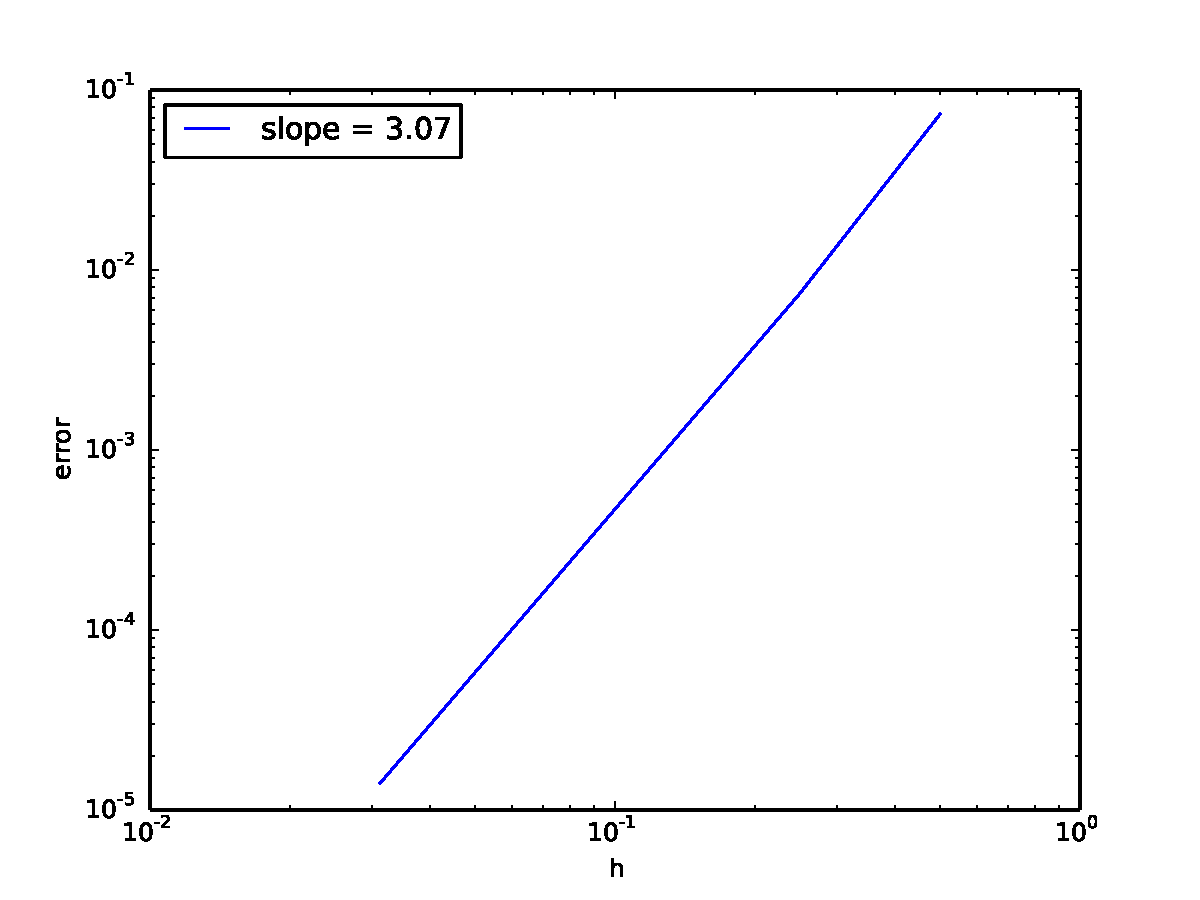
\includegraphics[width=0.7\textwidth]{SpaceTimeHeat/convergence}
	\caption{$L^2$ convergence of $u_1$ and $u_2$ for the 2D Burgers' equation}
	\label{fig:Burgers2DConvergence}
\end{figure}
\end{document}